% =====================================================================
% fig_gamification_architecture.tex
% ---------------------------------
% Editable TikZ architecture diagram for PECS Paper B §5.5
% (gamification layer of the f-SLA).  Mirrors FSLA_GAMIFICATION_VISION.md
% §3.1 and maps each block onto the SEANERGYS reference architecture
% (CMI + AIDAS + DSRM, vision §3.2).
%
% Compile standalone:
%   pdflatex --output-directory=. fig_gamification_architecture.tex
% or include with \includegraphics{fig_gamification_architecture}
% (a corresponding .pdf is produced by the standalone build).
% =====================================================================
\documentclass[border=4pt]{standalone}
\usepackage{tikz}
\usepackage{amsmath}
\usetikzlibrary{positioning,arrows.meta,calc,fit,backgrounds,shapes.geometric}

\definecolor{userBox}{HTML}{4A90E2}
\definecolor{opBox}{HTML}{F3A93F}
\definecolor{ledgerBox}{HTML}{6FC77A}
\definecolor{schedBox}{HTML}{C0504D}
\definecolor{seanerBox}{HTML}{8E7CC3}
\definecolor{lineGray}{HTML}{555555}

\begin{document}
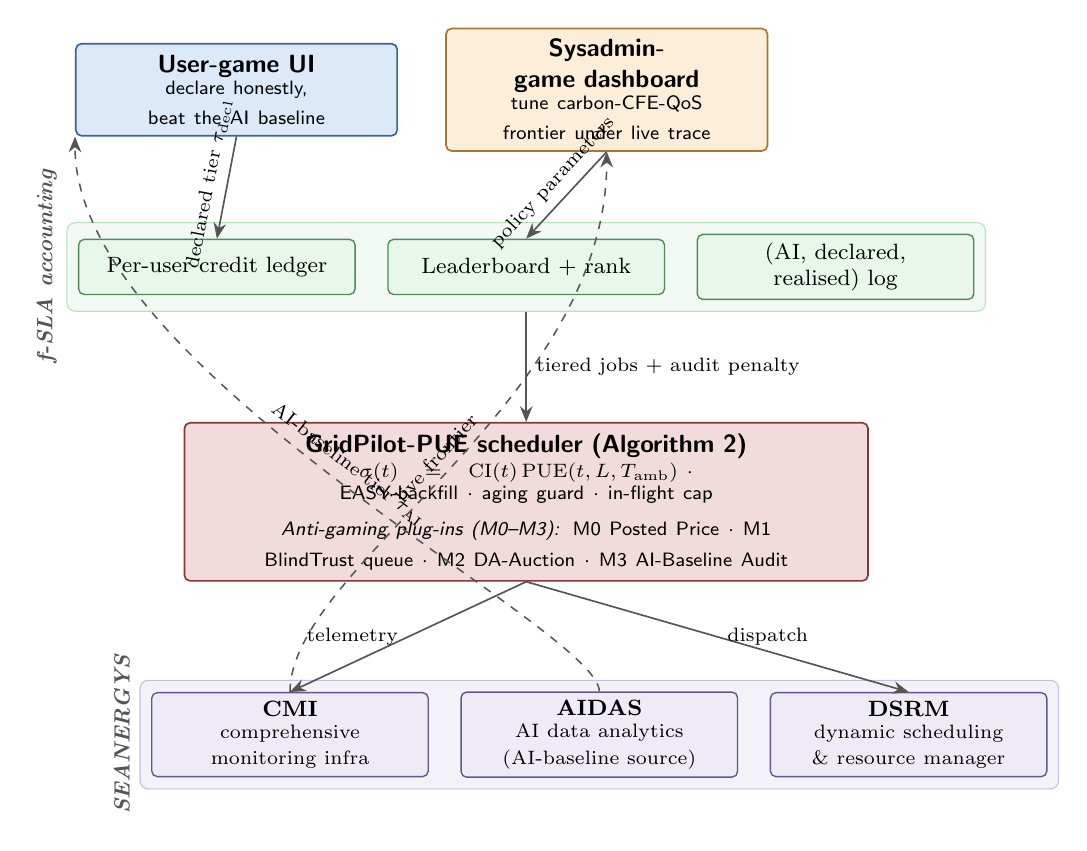
\begin{tikzpicture}[
  font=\sffamily\small,
  node distance=4mm and 6mm,
  >={Stealth[length=2mm,width=1.6mm]},
  box/.style={rectangle, rounded corners=2pt, draw=#1!70!black, fill=#1!20,
              line width=0.6pt, align=center, text width=38mm,
              inner sep=4pt, minimum height=9mm},
  smallbox/.style={rectangle, rounded corners=2pt, draw=#1!70!black, fill=#1!15,
                    line width=0.5pt, align=center, text width=33mm,
                    inner sep=3pt, minimum height=7mm, font=\footnotesize},
  flow/.style={->, draw=lineGray, line width=0.6pt},
  flowback/.style={->, dashed, draw=lineGray, line width=0.55pt},
  layerLabel/.style={font=\itshape\footnotesize, text=lineGray, anchor=west}
]

% ===== Layer 1 — user/operator front-end =============================
\node[box=userBox] (uig)
  {\textbf{User-game UI}\\\scriptsize declare honestly,\\\scriptsize beat the AI baseline};
\node[box=opBox, right=of uig] (sig)
  {\textbf{Sysadmin-game dashboard}\\\scriptsize tune carbon-CFE-QoS\\\scriptsize frontier under live trace};

% ===== Layer 2 — f-SLA accounting =====================================
\node[smallbox=ledgerBox, below=12mm of $(uig.south)!0.5!(sig.south)$, xshift=-26mm]
  (ledger) {Per-user credit ledger};
\node[smallbox=ledgerBox, right=4mm of ledger]
  (board) {Leaderboard + rank};
\node[smallbox=ledgerBox, right=4mm of board]
  (triplog) {(AI, declared, realised) log};

% Background box framing the accounting layer
\begin{scope}[on background layer]
  \node[rectangle, fill=ledgerBox!10, draw=ledgerBox!50,
        line width=0.4pt, rounded corners=3pt,
        fit=(ledger)(board)(triplog),
        inner xsep=4pt, inner ysep=4pt] (accbox) {};
\end{scope}
\node[layerLabel, anchor=east] at (accbox.west)
  {\rotatebox{90}{\textbf{f-SLA accounting}}};

% ===== Layer 3 — scheduler with mechanism plug-ins ===================
\node[box=schedBox, below=14mm of accbox.south,
       text width=84mm, minimum height=18mm]
  (sched)
  {\textbf{GridPilot-PUE scheduler (Algorithm 2)} \\[1pt]
   \scriptsize  $\sigma(t)=\mathrm{CI}(t)\,\mathrm{PUE}(t,L,T_{\mathrm{amb}})$  $\cdot$  EASY-backfill  $\cdot$  aging guard  $\cdot$  in-flight cap \\[2pt]
   \scriptsize \emph{Anti-gaming plug-ins (M0--M3):}
    M0 Posted Price  $\cdot$  M1 BlindTrust queue  $\cdot$  M2 DA-Auction  $\cdot$  M3 AI-Baseline Audit};

% ===== Layer 4 — SEANERGYS (CMI + AIDAS + DSRM) =====================
\node[smallbox=seanerBox, below=14mm of sched.south, xshift=-30mm,
       text width=33mm] (cmi)
  {\textbf{CMI}\\\scriptsize comprehensive\\\scriptsize monitoring infra};
\node[smallbox=seanerBox, right=4mm of cmi, text width=33mm] (aidas)
  {\textbf{AIDAS}\\\scriptsize AI data analytics\\\scriptsize (AI-baseline source)};
\node[smallbox=seanerBox, right=4mm of aidas, text width=33mm] (dsrm)
  {\textbf{DSRM}\\\scriptsize dynamic scheduling\\\scriptsize \& resource manager};

\begin{scope}[on background layer]
  \node[rectangle, fill=seanerBox!10, draw=seanerBox!50,
        line width=0.4pt, rounded corners=3pt,
        fit=(cmi)(aidas)(dsrm),
        inner xsep=4pt, inner ysep=4pt] (seanerBox) {};
\end{scope}
\node[layerLabel, anchor=east] at (seanerBox.west)
  {\rotatebox{90}{\textbf{SEANERGYS}}};

% ===== Arrows: front-end → accounting =====
\draw[flow] (uig.south)  -- node[midway, sloped, above, font=\scriptsize]
                                   {declared tier $\tau_{\mathrm{decl}}$} (ledger.north);
\draw[flow] (sig.south)  -- node[midway, sloped, above, font=\scriptsize]
                                   {policy parameters} (board.north);

% ===== Arrows: accounting → scheduler =====
\draw[flow] (accbox.south) -- node[midway, right, font=\scriptsize]
                                   {tiered jobs + audit penalty} (sched.north);

% ===== Arrows: scheduler → SEANERGYS =====
\draw[flow] (sched.south) -- node[midway, left, font=\scriptsize]
                                   {telemetry} (cmi.north);
\draw[flow] (sched.south) -- node[midway, right, font=\scriptsize]
                                   {dispatch} (dsrm.north);

% ===== AIDAS feedback to user UI (the AI baseline) =====
\draw[flowback] (aidas.north) .. controls +(0,8mm) and +(0,-30mm) ..
  node[midway, sloped, above, font=\scriptsize]
       {AI-baseline tier $\tau_{\mathrm{AI}}$} (uig.south west);

% ===== CMI feedback to operator dashboard =====
\draw[flowback] (cmi.north) .. controls +(0,16mm) and +(0,-32mm) ..
  node[midway, sloped, above, font=\scriptsize]
       {live frontier} (sig.south);

\end{tikzpicture}
\end{document}
